We now touch on lists (from Gaddis Chapter 7) and then go back to Chapters 4 and 5 to cover repetition structures and functions. 

\section{Lists}
\scalebox{0.8}{\textit{Reference: Gaddis Chapter 7}}

\subsection{Defining Lists (G\S 7.2)}

We have worked with strings, integers, floats, and booleans so far. Now, we introduce a compound data type the list.
Lists are also a sequence object, meaning they are ordered. 

A list is constructed by separating one or more objects with commas and placing them in square brackets. For example, we can define a list as follows.

\begin{lstlisting}[language = Python]
# Our first list---some Peloton content categories
floor = ['yoga', 'meditation', 'stretching', 'strength', 'cardiovascular'] \end{lstlisting}

\begin{lstlisting}[language = Python]
# More lists
aquatic = []
cycling = ['cycling'] \end{lstlisting}

\begin{lstlisting}[language = Python]
# More lists
treadmill_based = ['running', 'walking', 'bootcamp']  \end{lstlisting}

A useful quality of lists is that they can be of mixed type. 

\begin{lstlisting}[language = Python]
# More lists
fine_list = [0, 'milk', cycling]  \end{lstlisting}

\subsection{Indexing, Slicing, Mutating (G\S 7.2, 7.3)}

You can obtain the element at a certain place, or \emph{index}, in a list by suffixing the list with that index number inside square brackets. 
Python uses zero-based indexing. So one might say the $n^{\text{th}}$ item is at index $n-1$. This can create confusion when talking about the first, second, etc items in a list. I'll try always to speak of elements \emph{at index} zero, one, etc, so that you know I am referring to the position according to this zero-based system. 

\begin{lstlisting}[language = Python]
# Get specific items
fine_list = [0, 'milk', cycling]

# Which of these print statements will raise an error?
print(fine_list[0])
print(fine_list[1])
print(fine_list[2])
print(fine_list[3])
print(fine_list[-1])) \end{lstlisting}


We can also count from the end of the list to find an item, as hinted by the 
\code{fine_list[-1]} above. The index $-1$ will identify the last element. So, in some sense, you might say that negative indexing
is not zero-based though it is in fact consistent with the zero-based indexing described above. If that's confusing, recall $-0 = 0$ and so \code{fine_list[-0]} 
is actually the same as \code{fine_list[0]}.


The following graphic helps explain how lists (and strings) are indexed.

\begin{figure}[h!] 
\begin{center} 
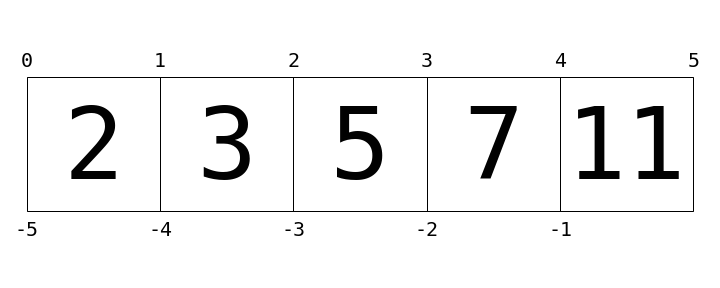
\includegraphics[width = .55\textwidth]{list_indexing.png}
\caption{Indexing (\textcolor{blue}{\href{https://jakevdp.github.io/WhirlwindTourOfPython/06-built-in-data-structures.html}{From \emph{Whirlwind Tour of Python} by Jake VanderPlas}}).}
\label{fig:while}
\end{center}
\end{figure}


%% Slicing

\bigskip

While indexing pulled out a single element, we can also \emph{slice} to pull out a sublist. 


\begin{lstlisting}[language = Python]
# Get specific items
['Jack', 'Jill', 'and', 'hill', 'over', 'ran', 'the']
print(fine_list[0:2])
print(fine_list[-2:]) \end{lstlisting}

The first print statement will print elements 0 and 1 in a list. The last print statement will print a list of just the last two elements.



%% Mutability 
\bigskip

Lists are \emph{mutable}, meaning that we can change their contents.


\begin{lstlisting}[language = Python]
# Get specific items
fine_list = [0, 'milk', cycling]
print(fine_list[0])
fine_list[0] = 1.0
print(fine_list[0]) \end{lstlisting}


\section{Repetition Structures}
\scalebox{0.8}{\textit{Reference: Gaddis Chapter 4}}

Repetition structures (loops) are one of the best justifications for moving from Excel to Python (though they are not unique to Python). A ``program''
in Excel is a serious of keystrokes and clicks. You might create a report for your company that is specific to one
market and you'll need to replicate the same report for a different market. Perhaps you could write a macro, but
I think you'll find working in Python to be easier. In Python, we can do this in a loop. We can have a program that makes the report and we
can iterate through the different markets to apply the program to each and create the specific reports (using a for loop).

\subsection{While Loops (G\S4.2)}
 
The \textbf{while loop} is a condition-controlled loop. Figure \ref{fig:while} illustrates the logic well. See also Figure 2 in Gaddis \S 4.2 (p. 163).

\begin{figure}[h!] 
\begin{center} 
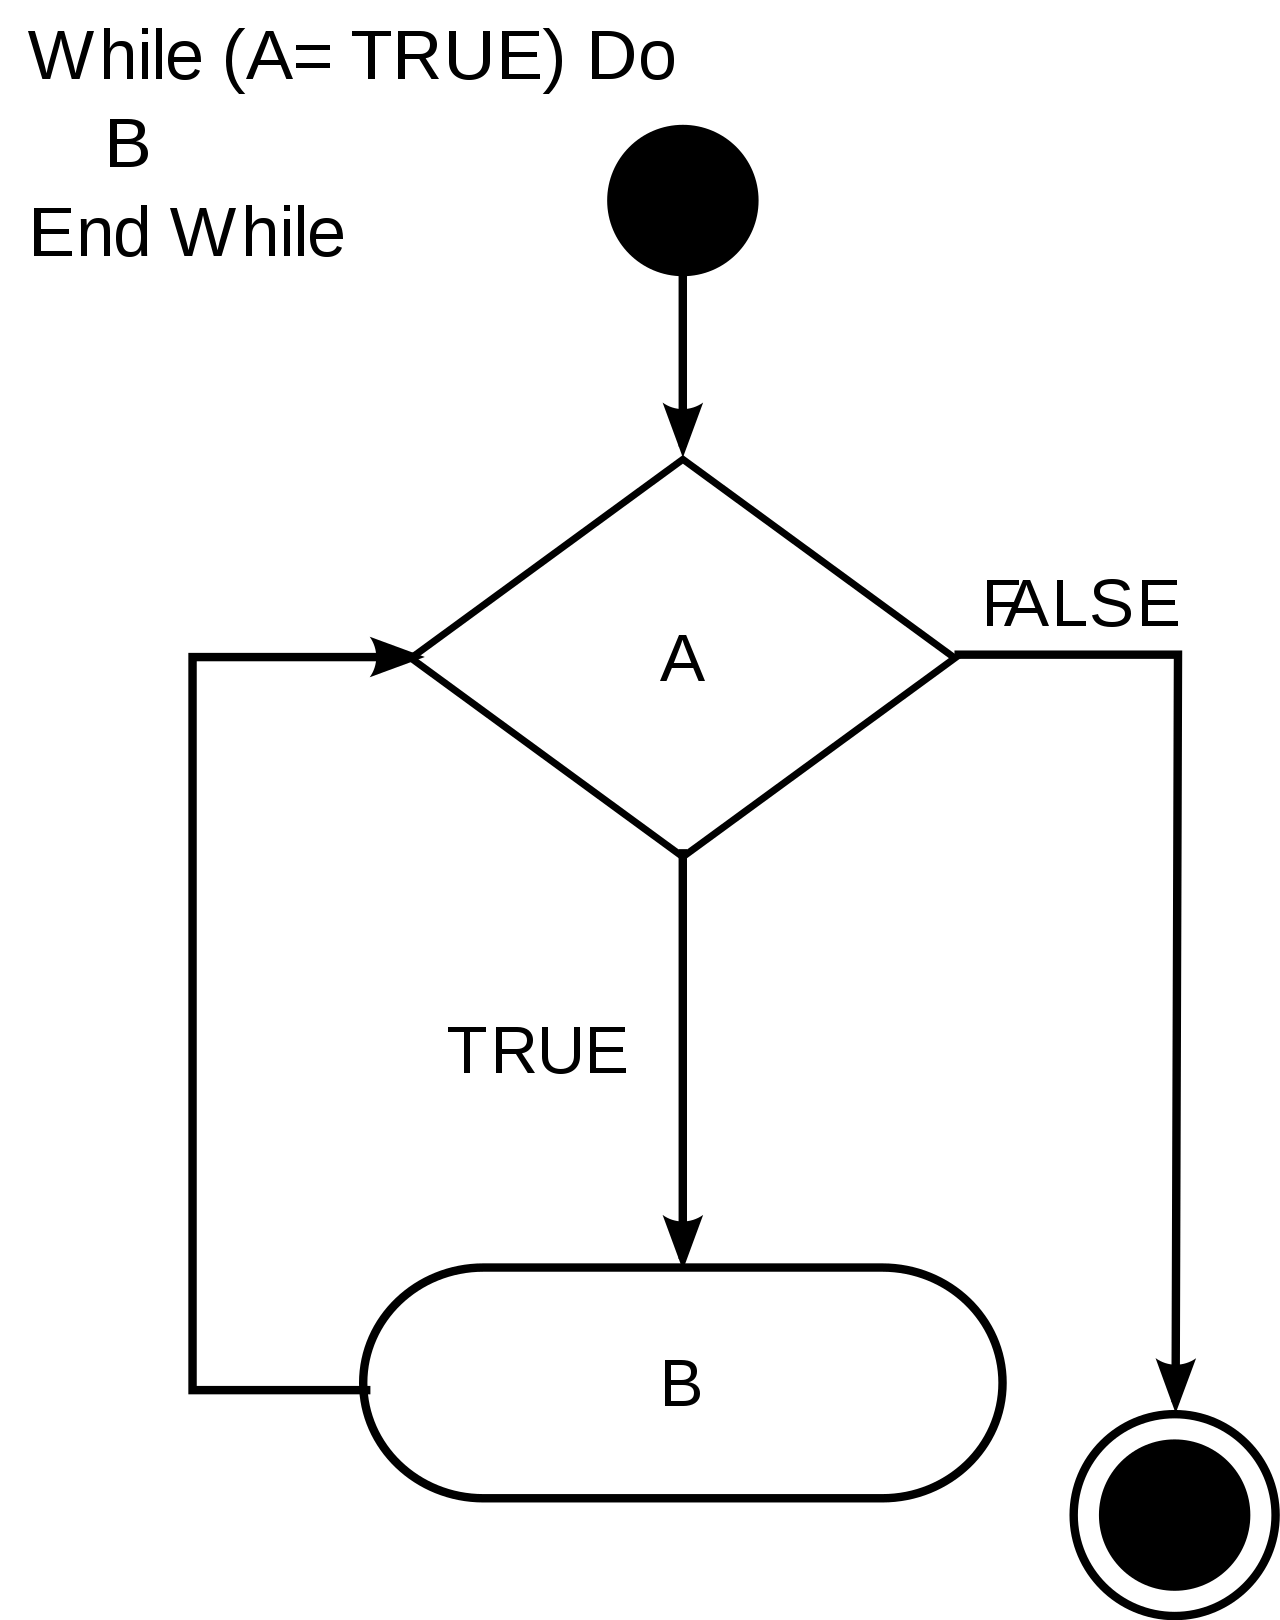
\includegraphics[width = .55\textwidth]{while_loop.png}
\caption{While loop logic (\textcolor{blue}{\href{https://en.wikipedia.org/wiki/While\_loop}{Wikipedia}}).}
\label{fig:while}
\end{center}
\end{figure}


The statement inside a while loop executes as long as the condition evaluates to True.

\begin{lstlisting}[language = Python]
# Rest on the seventh day
day_of_week = 1
while day_of_week < 7:
    print('work')
    day_of_week += 1 \end{lstlisting}


Beware the infinite loop. Be confident that your test condition will have a way of becoming False, otherwise
you might notice that your program never finishes. 


Let's consider an infinite series, $\sum_{i=0}^\infty 2^{-i} =  1 + \frac{1}{2} + \frac{1}{4} + \frac{1}{8} + \dots = 2$.
We could try to calculate this with a while loop if we didn't know the sum converged to two.

\begin{lstlisting}[language = Python]
# Sum of a geometric series
the_sum = 0
idx = 0
increment = 2 ** -idx

while increment > 0:
    # Increase the sum by the current increment
    the_sum += increment
    
    # Advance the index in the sum and calculate a new increment
    idx += 1
    increment = 2 ** (-idx) \end{lstlisting}
    

Does this loop make you nervous? In fact, the loop will terminate because we will eventually hit machine zero.
I found the loop to terminate at the increment $2^{-1075}$ and the resulting sum to be two. But it should make you nervous.
You might instead decide on some level of precision and use a test condition like 
\code{increment > .0005}, in which case you could find a bound on the error with some math.
Doing that math is not part of this course, (un)fortunately.


\subsection{For Loops (G\S4.3)} 
\label{sec:forloop}

For loops execute the attached code based on some iteration. The code might depend on a variable that is actually changing
with the iteration. 

\begin{lstlisting}[language = Python]
# Dr. Seuss
for item in [1,2,'red','blue']:
    print(item, 'fish')  \end{lstlisting}


The for clause tells Python to execute the statement once for every item in the iterable, which is in this case the object \code{[1,2,'red','blue']}. This is a \emph{list}, a kind of 
compound data object that can store other objects in sequence by separating them with commas and putting them inside square brackets. Below we use \code{range(5)} instead of a list, which you can think of as generating an iterable object of integers from 0 to 4 (5 is not included, but the length is 5).


\smallskip

Or you might just want to execute a specific set of statements some number of times.


\begin{lstlisting}[language = Python]
# Tubthumping by Chumbawamba
for item in range(5):
    print("I get knocked down, but I get up again.")
    print("You are never gonna keep me down.") \end{lstlisting}

\smallskip

For both of the examples above, \code{item} is the \emph{variable}. However, notice
the print statement only depends on the variable in the first example.

\smallskip
You can even iterate over the characters in a string.

\begin{lstlisting}[language = Python]
# Cheer
word = 'PYTHON'
for char in word:
    print("Give me a",char, '!')
    print("    ", char)
print("What's that spell?")
print("    ",word) \end{lstlisting}


\subsection{Nested Loops (G\S 4.7)}

A loop that is inside another is called \emph{nested}.

\smallskip
Think about how Python executes code line by line. What order of output do you expect from this program?


\begin{lstlisting}[language = Python]
# Nested Loop
for x in ['wee', 'bee']:
    for y in ['bop', 'dop']:
        print(x,y) \end{lstlisting}


\smallskip




\section{Functions}
\scalebox{0.8}{\textit{Reference: Gaddis Chapter 5}}

\emph{Functions} make your code easier to read and reuse by performing a certain task based on some number of arguments
the function takes. 

In math, you might define a function $f(x) = x^2$. Just as $f$ does something with $x$, a function like 
\lstinline[language=Python]{print} does something with whatever input we pass inside the parentheses.

Consider the cheer we made in Section \ref{sec:forloop}. 

\begin{lstlisting}[language = Python]
# Cheer
word = 'PYTHON'
for char in word:
    print("Give me a",char, '!')
    print("    ", char)
print("What's that spell?")
print("    ",word) \end{lstlisting}


We can make this into a function. 


\begin{lstlisting}[language = Python]
# Cheer Function
def cheer(word):
    ''' Doc string '''
    for char in word:
        print("Give me a",char, '!')
        print("    ", char)
    print("What's that spell?")
    print("    ",word) \end{lstlisting}
    
Here's another function that takes a number and returns the next multiple of five by making use of a while loop. This is our first \emph{value-returning} function. Don't confuse the idea of a function returning something with simply doing something. The \code{cheer} function merely did something by printing a cheer. 

\begin{lstlisting}[language = Python]
# Find a nearby multiple of five
def find_close_multiple_of_five(num):
    # check if multiple of five
    is_multiple = num % 5 == 0
    while is_multiple not True:
        num += 1
        is_multiple = num % 5
    return num \end{lstlisting}
    
\section{Exercise}

\textbf{Hard}: Write a program that will find the first prime number after some given integer.

\vfill

\textit{Answers on next page.}

\pagebreak


\subsection{Exercise Answers}


\textbf{Hard}: Write a program that will find the first prime number after some given integer.

\begin{lstlisting}[language = Python]
# Find the first prime number greater than num.
# Initialize with a composite number
num = 20
is_prime = False

# Incremement the number until we find a prime.
while is_prime == False:
    num += 1
    is_prime = True # Initialize as prime and overwrite later
    
    for divisor in range(2,num): # Checks all integers >=2 and < num 
        if num % divisor == 0: # We enter the if statement when num/divisor is a whole number
            is_prime = False and is_prime # False along with and will make the whole boolean False
    # is_prime remains True when we exit the for loop not having found a single divisor \end{lstlisting}